\section{Profiling- und Performance-Tests}
Um einen Überblick über den Zeitaufwand der einzelnen Worthwhile-Komponenten zu gewinnen sowie zeitliche Hotspots zu identifizieren, wurden Profiling-Tests mit Unterstützung von VisualVM durchgeführt. Hierbei wurden einzelne, meist komplexere, Testprogramme aus der GUI gestartet und untersucht, um einen Eindruck von Worthwhile unter möglichst realen Bedingungen zu erlangen.

\subsection{Parser}
Das Parsen eines Programms ist abhängig von der Anzahl der vorkommenden Sprachkonstrukte. Beispielsweise dauerte das Parsen des Programms \texttt{bubblesort2.ww} 111~Millisekunden~(ms) . Eine eindeutige Aussage über die Dauer eines Parse-Vorgangs lässt sich schwer treffen, da die Anzahl sowie die Verschachtelungstiefe der Sprachkonstrukte eine große Rolle spielen. Jedoch benötigen die einzelnen Sprachkonstrukte eine Bearbeitungszeit von Millisekunden-Bruchteilen bis hin zu wenigen Millisekunden. Im Testprogramm \texttt{bubblesort2.ww} stellte sich die Funktionsdeklaration mit 5,56~ms als am zeitaufwendigsten heraus.

\subsection{Interpreter}
Der Zeitbedarf für das Interpretieren ist genauso wie das Parsen abhängig von der Anzahl der Sprachkonstrukte. Jedoch muss hier nicht die Anzahl der vorkommenden, sondern die der auszuführenden Elemente berücksichtigt werden. Deshalb lässt sich auch hier nicht eindeutig sagen, wie viel Zeit ein Programm in der Ausführung benötigt, da insbesondere ein Prorgamm unter Umständen nie terminiert. Das Sortieren eines Arrays mit zehn Elementen mittels \texttt{bubblesort2.ww} benötigte etwa 18~Sekunden~(s). Diese relativ hohe Zeit ist auf die ständig auftretenden Beweiseraufrufe zurückzuführen, welche annähernd 100\% der Zeit ausmachten. Das Sortieren ohne die Beweiseraufrufe dauerte ca. 26~ms.

\subsection{Prover}
Das Überprüfen eines Testprogramms dauerte im Schnitt etwa 2~s. Am Beispiel der Testprogramme \texttt{test\_fibonacci.ww} und \texttt{bubblesort2.ww} lag die Beweiszeit bei 1865~ms bzw. 1895~ms. Da vor dem Beweisen ein Parsen des Codes und Typsystemüberprüfungen nötig sind, fallen etwa 100~ms bis 200~ms auf diese Aufgaben zurück. Die Transformation des Codes im wp-Kalkül benötigte für \texttt{bubblesort2.ww} 142~ms und für \texttt{test\_fibonacci.ww} 36~ms. Das Umwandeln einer einzelnen Annotation ins SMTLIB-Format betrug bei beiden Tests wenige Millisekunden (im Schnitt etwa 4~ms). Da jedoch die Annotationen einzeln umgewandelt und überprüft werden, liegt die Gesamtzeit der Umwandlungen ins SMTLIB-Format deutlich höher. Das Testprogramm \texttt{bubblesort2.ww} enthielt 13 und \texttt{test\_fibonacci.ww} 11 zu überprüfende Annotationen. Somit liegt der Zeitbedarf für das Umwandeln aller Annotation bei etwa 50~ms. Ebenso wird jede Annotation anschließend mittels externem Beweiser überprüft. Einzelne Annotationen zu beweisen, dauerte etwa 15~ms bis 17~ms und demnach lag der Gesamtzeitaufwand des Beweisers für das gesamte Programm bei 220~ms für \texttt{bubblesort2.ww} und bei 170~ms für \texttt{test\_fibonacci.ww}. Nach Überprüfung weiterer Testprogramme ergibt sich somit ein ungefährer Überblick über den anteiligen Zeitaufwand der Prover-Komponenten in Tabelle~\ref{zeitaufwandprover}.

\begin{table}
\centering
\caption{Ungefährer Zeitaufwand der Prover-Komponenten}
\label{zeitaufwandprover}
\begin{tabular}{|l|l|}
\hline
\textbf{Komponente} & \textbf{Zeitaufwand} \\
\hline
Parser und Typsystem & 10\% \\
\hline
wp-Kalkül & 8\% \\
\hline
SMTLIB-Formatierung & 4\% \\
\hline
Beweiser (Z3) & 15\% \\
\hline
\end{tabular}
\end{table}

\subsection{Ressourcen}
Der Speicherverbrauch für den Heap von Worthwhile liegt aufgrund der Eclipse-Umgebung bei etwa 45 MB (siehe Abbildung \ref{heapsize}). Die Anzahl der Threads liegt im Idle-Modus bei etwa 28 Threads und steigt leicht beim Ausführen bzw. Beweisen eines Programms (siehe Abbildung \ref{threadcount}). Die CPU-Last steigt beim Start des Programms auf etwa 30\% (siehe 4:18:40 PM in Abbildung \ref{cpuusage}) und verhält sich sonst bei unter 5\%. Beim Beweisen eines Programms steigt sie kurzzeitig auf ebenfalls etwa 30\% (4:18:55 PM in Abbildung \ref{cpuusage}). Diese Werte sind trotz der Benutzung großer und mächtiger Bibliotheken wie XText völlig ausreichend, um eine flüssige Benutzung auf aktuellen Systemen zu gewährleisten.

\begin{center}
	\begin{figure}
		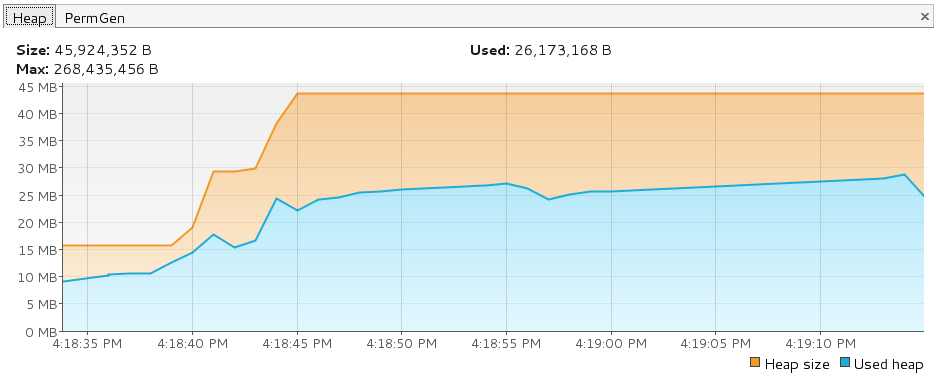
\includegraphics[width=13cm]{images/worthwhile-ressourcen-heap.png}
		\caption{Speicherverbrauch von worthwhile}
 		\label{heapsize}
	\end{figure}
\end{center}

\begin{center}
	\begin{figure}[h]
		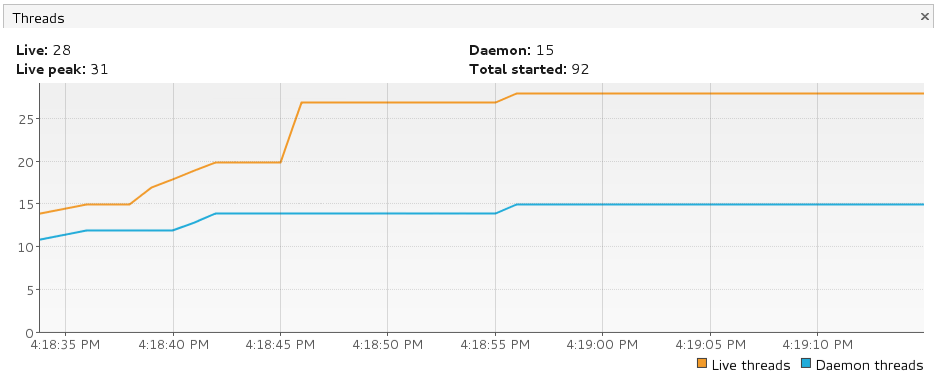
\includegraphics[width=13cm]{images/worthwhile-ressourcen-threads.png}
		\caption{Anzahl der Threads}
 		\label{threadcount}
	\end{figure}
\end{center}

\begin{center}
	\begin{figure}[h]
		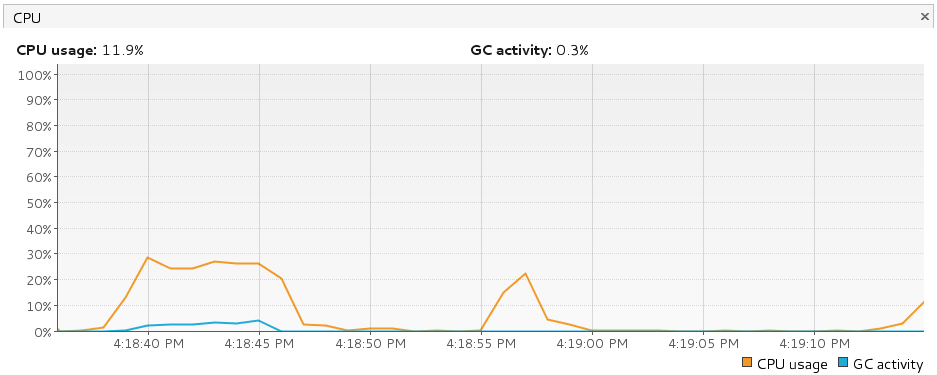
\includegraphics[width=13cm]{images/worthwhile-ressourcen-cpu.png}
		\caption{CPU Auslastung}
 		\label{cpuusage}
	\end{figure}
\end{center}
